\documentclass{article}
\usepackage{amsmath}
\usepackage{amsfonts}
\usepackage{amssymb}
\usepackage{tikz}
\usepackage{caption}
\usepackage{subcaption}

\begin{document}

\begin{figure}[!ht]
    \centering
    \begin{subfigure}{0.48\textwidth}
        \centering
        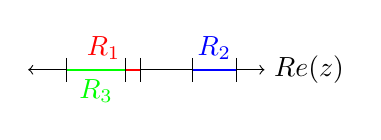
\begin{tikzpicture}[scale=1.5]
            \draw[<->] (-1.2,0) -- (0.8,0) node[right] {$Re(z)$};

            % Disks R1, R2, R3
            \draw[red, thick] (-0.875,0) -- (-0.25,0);
            \node[red, above] at (-0.5625,0) {$R_1$};

            \draw[blue, thick] (0.1875,0) -- (0.5625,0);
            \node[blue, above] at (0.375,0) {$R_2$};

            \draw[green, thick] (-0.875,0) -- (-0.375,0);
            \node[green, below] at (-0.625,0) {$R_3$};

            %Marking Intervals to ensure good visual check.
            \foreach \x in {-0.875, -0.25, 0.1875, 0.5625, -0.375}
                \draw (\x,0.1) -- (\x,-0.1);

        \end{tikzpicture}
        \caption{Disks $R_1$, $R_2$, $R_3$}
        \label{fig:gershgorin_1}
    \end{subfigure}%
    \hfill%
    \begin{subfigure}{0.48\textwidth}
        \centering
        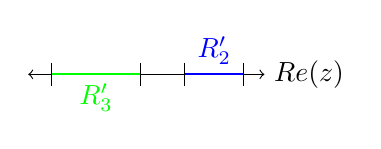
\begin{tikzpicture}[scale=1.5]
            \draw[<->] (-1.2,0) -- (0.8,0) node[right] {$Re(z)$};

            % Disks R1', R2', R3'
            % \draw[red, thick] (-0.6875,0) -- (-0.3125,0);
            % \node[red, above] at (-0.5,0) {$R_1'$}; %Removed This

            \draw[blue, thick] (0.125,0) -- (0.625,0);
            \node[blue, above] at (0.375,0) {$R_2'$};

            \draw[green, thick] (-1,0) -- (-0.25,0);
            \node[green, below] at (-0.625,0) {$R_3'$};

            %Marking Intervals to ensure good visual check.
            \foreach \x in {0.125, 0.625, -1, -0.25} %Removed the now irrelevant points
                \draw (\x,0.1) -- (\x,-0.1);

        \end{tikzpicture}
        \caption{Disks $R_2'$, $R_3'$ (Since R1' is a subset of R3')}
        \label{fig:gershgorin_2}
    \end{subfigure}
    \caption{Gershgorin Disks}
    \label{fig:gershgorin_all}
\end{figure}

\end{document}